\documentclass[1p]{elsarticle_modified}
%\bibliographystyle{elsarticle-num}

%\usepackage[colorlinks]{hyperref}
%\usepackage{abbrmath_seonhwa} %\Abb, \Ascr, \Acal ,\Abf, \Afrak
\usepackage{amsfonts}
\usepackage{amssymb}
\usepackage{amsmath}
\usepackage{amsthm}
\usepackage{scalefnt}
\usepackage{amsbsy}
\usepackage{kotex}
\usepackage{caption}
\usepackage{subfig}
\usepackage{color}
\usepackage{graphicx}
\usepackage{xcolor} %% white, black, red, green, blue, cyan, magenta, yellow
\usepackage{float}
\usepackage{setspace}
\usepackage{hyperref}

\usepackage{tikz}
\usetikzlibrary{arrows}

\usepackage{multirow}
\usepackage{array} % fixed length table
\usepackage{hhline}

%%%%%%%%%%%%%%%%%%%%%
\makeatletter
\renewcommand*\env@matrix[1][\arraystretch]{%
	\edef\arraystretch{#1}%
	\hskip -\arraycolsep
	\let\@ifnextchar\new@ifnextchar
	\array{*\c@MaxMatrixCols c}}
\makeatother %https://tex.stackexchange.com/questions/14071/how-can-i-increase-the-line-spacing-in-a-matrix
%%%%%%%%%%%%%%%

\usepackage[normalem]{ulem}

\newcommand{\msout}[1]{\ifmmode\text{\sout{\ensuremath{#1}}}\else\sout{#1}\fi}
%SOURCE: \msout is \stkout macro in https://tex.stackexchange.com/questions/20609/strikeout-in-math-mode

\newcommand{\cancel}[1]{
	\ifmmode
	{\color{red}\msout{#1}}
	\else
	{\color{red}\sout{#1}}
	\fi
}

\newcommand{\add}[1]{
	{\color{blue}\uwave{#1}}
}

\newcommand{\replace}[2]{
	\ifmmode
	{\color{red}\msout{#1}}{\color{blue}\uwave{#2}}
	\else
	{\color{red}\sout{#1}}{\color{blue}\uwave{#2}}
	\fi
}

\newcommand{\Sol}{\mathcal{S}} %segment
\newcommand{\D}{D} %diagram
\newcommand{\A}{\mathcal{A}} %arc


%%%%%%%%%%%%%%%%%%%%%%%%%%%%%5 test

\def\sl{\operatorname{\textup{SL}}(2,\Cbb)}
\def\psl{\operatorname{\textup{PSL}}(2,\Cbb)}
\def\quan{\mkern 1mu \triangleright \mkern 1mu}

\theoremstyle{definition}
\newtheorem{thm}{Theorem}[section]
\newtheorem{prop}[thm]{Proposition}
\newtheorem{lem}[thm]{Lemma}
\newtheorem{ques}[thm]{Question}
\newtheorem{cor}[thm]{Corollary}
\newtheorem{defn}[thm]{Definition}
\newtheorem{exam}[thm]{Example}
\newtheorem{rmk}[thm]{Remark}
\newtheorem{alg}[thm]{Algorithm}

\newcommand{\I}{\sqrt{-1}}
\begin{document}

%\begin{frontmatter}
%
%\title{Boundary parabolic representations of knots up to 8 crossings}
%
%%% Group authors per affiliation:
%\author{Yunhi Cho} 
%\address{Department of Mathematics, University of Seoul, Seoul, Korea}
%\ead{yhcho@uos.ac.kr}
%
%
%\author{Seonhwa Kim} %\fnref{s_kim}}
%\address{Center for Geometry and Physics, Institute for Basic Science, Pohang, 37673, Korea}
%\ead{ryeona17@ibs.re.kr}
%
%\author{Hyuk Kim}
%\address{Department of Mathematical Sciences, Seoul National University, Seoul 08826, Korea}
%\ead{hyukkim@snu.ac.kr}
%
%\author{Seokbeom Yoon}
%\address{Department of Mathematical Sciences, Seoul National University, Seoul, 08826,  Korea}
%\ead{sbyoon15@snu.ac.kr}
%
%\begin{abstract}
%We find all boundary parabolic representation of knots up to 8 crossings.
%
%\end{abstract}
%\begin{keyword}
%    \MSC[2010] 57M25 
%\end{keyword}
%
%\end{frontmatter}

%\linenumbers
%\tableofcontents
%
\newcommand\colored[1]{\textcolor{white}{\rule[-0.35ex]{0.8em}{1.4ex}}\kern-0.8em\color{red} #1}%
%\newcommand\colored[1]{\textcolor{white}{ #1}\kern-2.17ex	\textcolor{white}{ #1}\kern-1.81ex	\textcolor{white}{ #1}\kern-2.15ex\color{red}#1	}

{\Large $\underline{12n_{0120}~(K12n_{0120})}$}

\setlength{\tabcolsep}{10pt}
\renewcommand{\arraystretch}{1.6}
\vspace{1cm}\begin{tabular}{m{100pt}>{\centering\arraybackslash}m{274pt}}
\multirow{5}{120pt}{
	\centering
	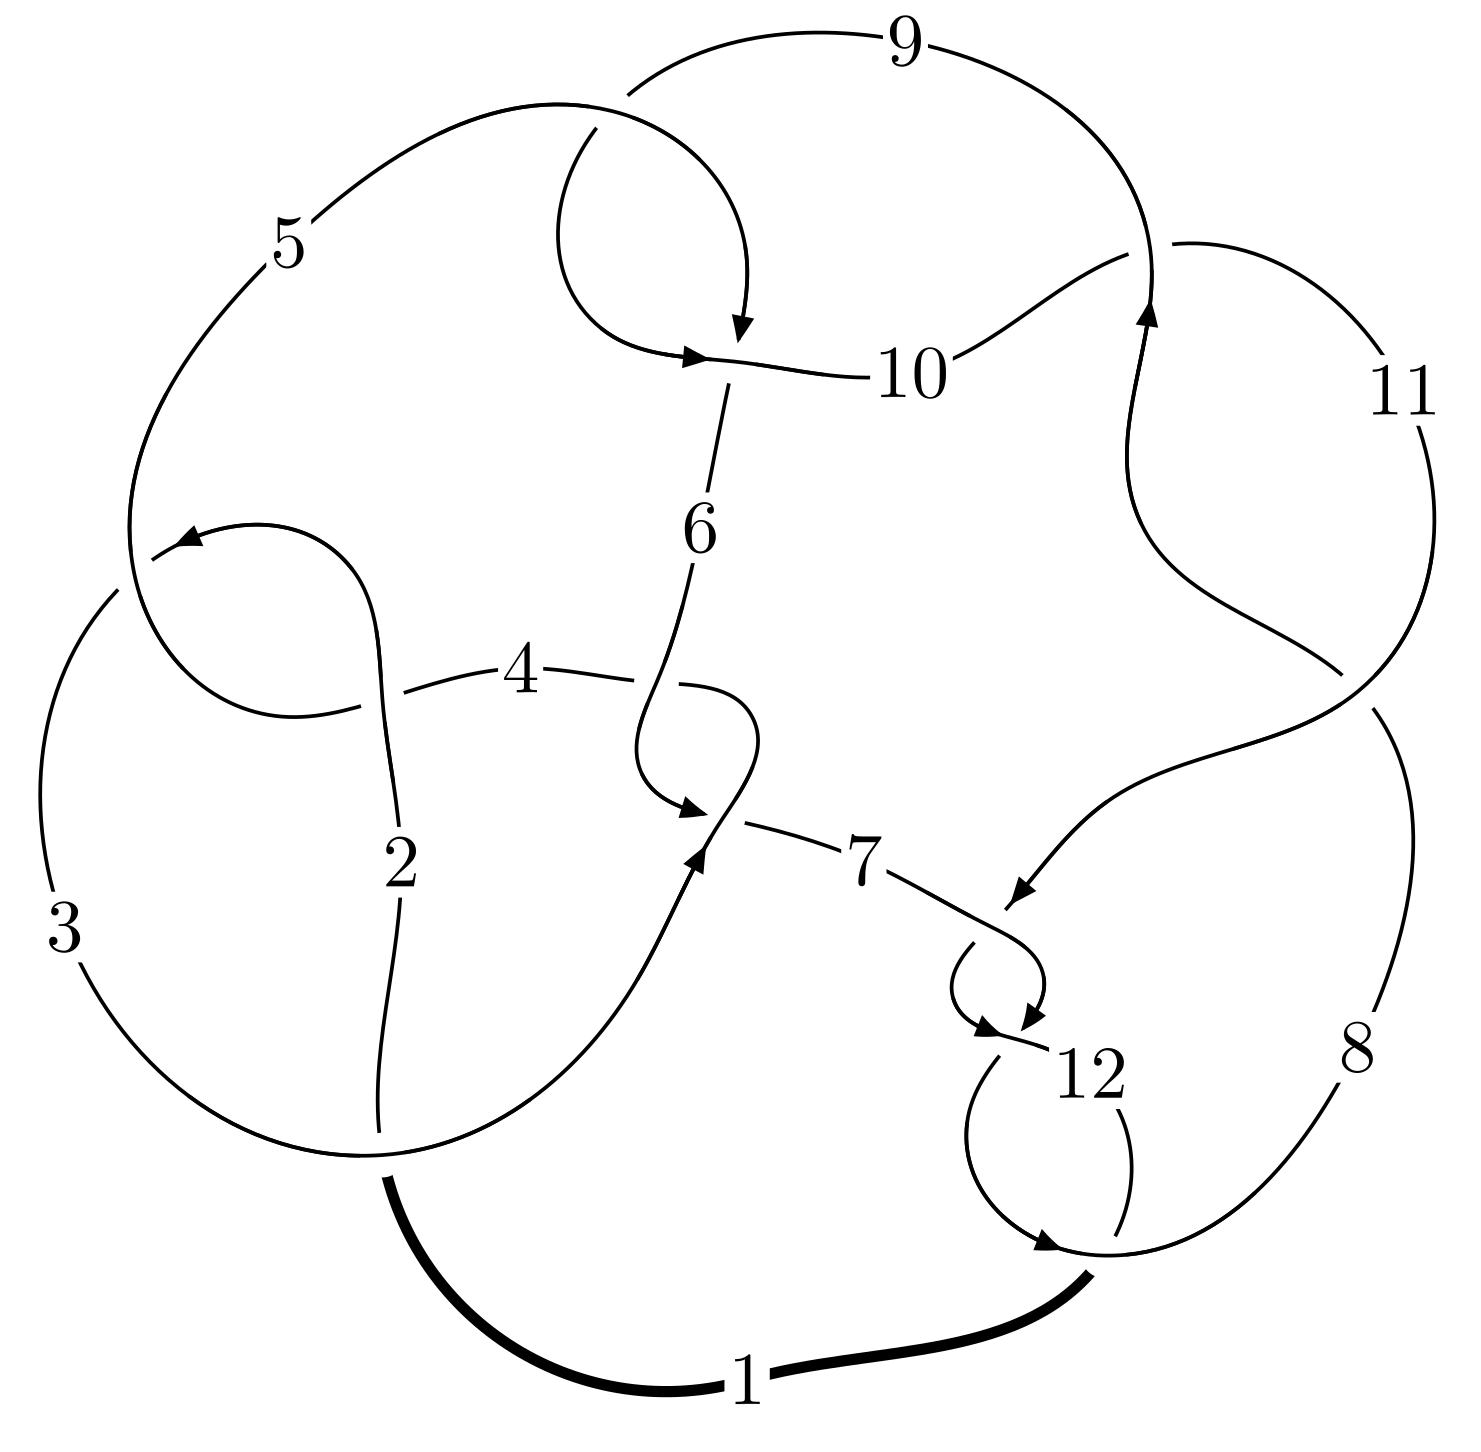
\includegraphics[width=112pt]{../../../GIT/diagram.site/Diagrams/png/2209_12n_0120.png}\\
\ \ \ A knot diagram\footnotemark}&
\allowdisplaybreaks
\textbf{Linearized knot diagam} \\
\cline{2-2}
 &
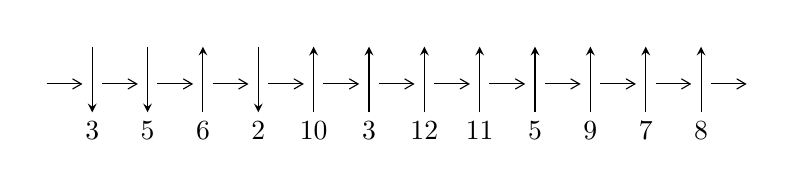
\begin{tikzpicture}[x=20pt, y=17pt]
	% nodes
	\node (C0) at (0, 0) {};
	\node (C1) at (1, 0) {};
	\node (C1U) at (1, +1) {};
	\node (C1D) at (1, -1) {3};

	\node (C2) at (2, 0) {};
	\node (C2U) at (2, +1) {};
	\node (C2D) at (2, -1) {5};

	\node (C3) at (3, 0) {};
	\node (C3U) at (3, +1) {};
	\node (C3D) at (3, -1) {6};

	\node (C4) at (4, 0) {};
	\node (C4U) at (4, +1) {};
	\node (C4D) at (4, -1) {2};

	\node (C5) at (5, 0) {};
	\node (C5U) at (5, +1) {};
	\node (C5D) at (5, -1) {10};

	\node (C6) at (6, 0) {};
	\node (C6U) at (6, +1) {};
	\node (C6D) at (6, -1) {3};

	\node (C7) at (7, 0) {};
	\node (C7U) at (7, +1) {};
	\node (C7D) at (7, -1) {12};

	\node (C8) at (8, 0) {};
	\node (C8U) at (8, +1) {};
	\node (C8D) at (8, -1) {11};

	\node (C9) at (9, 0) {};
	\node (C9U) at (9, +1) {};
	\node (C9D) at (9, -1) {5};

	\node (C10) at (10, 0) {};
	\node (C10U) at (10, +1) {};
	\node (C10D) at (10, -1) {9};

	\node (C11) at (11, 0) {};
	\node (C11U) at (11, +1) {};
	\node (C11D) at (11, -1) {7};

	\node (C12) at (12, 0) {};
	\node (C12U) at (12, +1) {};
	\node (C12D) at (12, -1) {8};
	\node (C13) at (13, 0) {};

	% arrows
	\draw[->,>={angle 60}]
	(C0) edge (C1) (C1) edge (C2) (C2) edge (C3) (C3) edge (C4) (C4) edge (C5) (C5) edge (C6) (C6) edge (C7) (C7) edge (C8) (C8) edge (C9) (C9) edge (C10) (C10) edge (C11) (C11) edge (C12) (C12) edge (C13) ;	\draw[->,>=stealth]
	(C1U) edge (C1D) (C2U) edge (C2D) (C3D) edge (C3U) (C4U) edge (C4D) (C5D) edge (C5U) (C6D) edge (C6U) (C7D) edge (C7U) (C8D) edge (C8U) (C9D) edge (C9U) (C10D) edge (C10U) (C11D) edge (C11U) (C12D) edge (C12U) ;
	\end{tikzpicture} \\
\hhline{~~} \\& 
\textbf{Solving Sequence} \\ \cline{2-2} 
 &
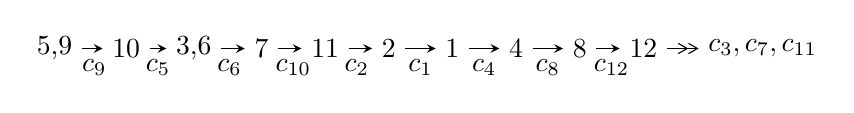
\begin{tikzpicture}[x=23pt, y=7pt]
	% node
	\node (A0) at (-1/8, 0) {5,9};
	\node (A1) at (1, 0) {10};
	\node (A2) at (33/16, 0) {3,6};
	\node (A3) at (25/8, 0) {7};
	\node (A4) at (33/8, 0) {11};
	\node (A5) at (41/8, 0) {2};
	\node (A6) at (49/8, 0) {1};
	\node (A7) at (57/8, 0) {4};
	\node (A8) at (65/8, 0) {8};
	\node (A9) at (73/8, 0) {12};
	\node (C1) at (1/2, -1) {$c_{9}$};
	\node (C2) at (3/2, -1) {$c_{5}$};
	\node (C3) at (21/8, -1) {$c_{6}$};
	\node (C4) at (29/8, -1) {$c_{10}$};
	\node (C5) at (37/8, -1) {$c_{2}$};
	\node (C6) at (45/8, -1) {$c_{1}$};
	\node (C7) at (53/8, -1) {$c_{4}$};
	\node (C8) at (61/8, -1) {$c_{8}$};
	\node (C9) at (69/8, -1) {$c_{12}$};
	\node (A10) at (11, 0) {$c_{3},c_{7},c_{11}$};

	% edge
	\draw[->,>=stealth]	
	(A0) edge (A1) (A1) edge (A2) (A2) edge (A3) (A3) edge (A4) (A4) edge (A5) (A5) edge (A6) (A6) edge (A7) (A7) edge (A8) (A8) edge (A9) ;
	\draw[->>,>={angle 60}]	
	(A9) edge (A10);
\end{tikzpicture} \\ 

\end{tabular} \\

\footnotetext{
The image of knot diagram is generated by the software ``\textbf{Draw programme}" developed by Andrew Bartholomew(\url{http://www.layer8.co.uk/maths/draw/index.htm\#Running-draw}), where we modified some parts for our purpose(\url{https://github.com/CATsTAILs/LinksPainter}).
}\phantom \\ \newline 
\centering \textbf{Ideals for irreducible components\footnotemark of $X_{\text{par}}$} 
 
\begin{align*}
I^u_{1}&=\langle 
15121 u^{16}-24215 u^{15}+\cdots+18155 b-26228,\;15121 u^{16}-24215 u^{15}+\cdots+18155 a-26228,\\
\phantom{I^u_{1}}&\phantom{= \langle  }u^{17}-2 u^{16}+2 u^{15}+7 u^{13}-14 u^{12}+14 u^{11}-2 u^{10}+7 u^9-14 u^8+14 u^7-12 u^6-2 u^2- u+1\rangle \\
I^u_{2}&=\langle 
- u^7+u^6+u^5-2 u^4- u^3+2 u^2+b+u-2,\;- u^7+u^6+u^5-2 u^4- u^3+2 u^2+a-2,\\
\phantom{I^u_{2}}&\phantom{= \langle  }u^8- u^7- u^6+2 u^5+u^4-2 u^3+2 u-1\rangle \\
\\
\end{align*}
\raggedright * 2 irreducible components of $\dim_{\mathbb{C}}=0$, with total 25 representations.\\
\footnotetext{All coefficients of polynomials are rational numbers. But the coefficients are sometimes approximated in decimal forms when there is not enough margin.}
\newpage
\renewcommand{\arraystretch}{1}
\centering \section*{I. $I^u_{1}= \langle 15121 u^{16}-24215 u^{15}+\cdots+18155 b-26228,\;15121 u^{16}-24215 u^{15}+\cdots+18155 a-26228,\;u^{17}-2 u^{16}+\cdots- u+1 \rangle$}
\flushleft \textbf{(i) Arc colorings}\\
\begin{tabular}{m{7pt} m{180pt} m{7pt} m{180pt} }
\flushright $a_{5}=$&$\begin{pmatrix}0\\u\end{pmatrix}$ \\
\flushright $a_{9}=$&$\begin{pmatrix}1\\0\end{pmatrix}$ \\
\flushright $a_{10}=$&$\begin{pmatrix}1\\- u^2\end{pmatrix}$ \\
\flushright $a_{3}=$&$\begin{pmatrix}-0.832884 u^{16}+1.33379 u^{15}+\cdots+1.24985 u+1.44467\\-0.832884 u^{16}+1.33379 u^{15}+\cdots+2.24985 u+1.44467\end{pmatrix}$ \\
\flushright $a_{6}=$&$\begin{pmatrix}u\\- u^3+u\end{pmatrix}$ \\
\flushright $a_{7}=$&$\begin{pmatrix}0.102561 u^{16}+0.104654 u^{15}+\cdots-0.0345359 u-0.615037\\0.0863674 u^{16}+0.0881300 u^{15}+\cdots-0.0290829 u-0.623189\end{pmatrix}$ \\
\flushright $a_{11}=$&$\begin{pmatrix}- u^2+1\\- u^2\end{pmatrix}$ \\
\flushright $a_{2}=$&$\begin{pmatrix}-0.832884 u^{16}+1.33379 u^{15}+\cdots+1.24985 u+1.44467\\-0.830185 u^{16}+1.33655 u^{15}+\cdots+1.74894 u+1.11270\end{pmatrix}$ \\
\flushright $a_{1}=$&$\begin{pmatrix}0.368438 u^{16}-0.644451 u^{15}+\cdots+0.212669 u-0.317929\\0.471000 u^{16}-0.539796 u^{15}+\cdots+0.178133 u-0.932966\end{pmatrix}$ \\
\flushright $a_{4}=$&$\begin{pmatrix}-0.816690 u^{16}+1.35032 u^{15}+\cdots+1.24440 u+1.45282\\-0.719526 u^{16}+1.44946 u^{15}+\cdots+2.21168 u+1.50174\end{pmatrix}$ \\
\flushright $a_{8}=$&$\begin{pmatrix}u^4- u^2+1\\u^4\end{pmatrix}$ \\
\flushright $a_{12}=$&$\begin{pmatrix}-0.167337 u^{16}-0.170752 u^{15}+\cdots+0.0563481 u+0.582429\\-0.140347 u^{16}-0.143211 u^{15}+\cdots+0.0472597 u-0.737318\end{pmatrix}$\\&\end{tabular}
\flushleft \textbf{(ii) Obstruction class $= -1$}\\~\\
\flushleft \textbf{(iii) Cusp Shapes $= -\frac{116556}{18155} u^{16}+\frac{32086}{3631} u^{15}+\cdots+\frac{186341}{18155} u+\frac{375193}{18155}$}\\~\\
\newpage\renewcommand{\arraystretch}{1}
\flushleft \textbf{(iv) u-Polynomials at the component}\newline \\
\begin{tabular}{m{50pt}|m{274pt}}
Crossings & \hspace{64pt}u-Polynomials at each crossing \\
\hline $$\begin{aligned}c_{1}\end{aligned}$$&$\begin{aligned}
&u^{17}+37 u^{16}+\cdots+129 u+1
\end{aligned}$\\
\hline $$\begin{aligned}c_{2},c_{4}\end{aligned}$$&$\begin{aligned}
&u^{17}-9 u^{16}+\cdots-9 u+1
\end{aligned}$\\
\hline $$\begin{aligned}c_{3},c_{6}\end{aligned}$$&$\begin{aligned}
&u^{17}+3 u^{16}+\cdots+1664 u-256
\end{aligned}$\\
\hline $$\begin{aligned}c_{5},c_{9}\end{aligned}$$&$\begin{aligned}
&u^{17}+2 u^{16}+\cdots- u-1
\end{aligned}$\\
\hline $$\begin{aligned}c_{7},c_{11},c_{12}\end{aligned}$$&$\begin{aligned}
&u^{17}+2 u^{16}+\cdots- u+1
\end{aligned}$\\
\hline $$\begin{aligned}c_{8},c_{10}\end{aligned}$$&$\begin{aligned}
&u^{17}+18 u^{15}+\cdots+5 u-1
\end{aligned}$\\
\hline
\end{tabular}\\~\\
\newpage\renewcommand{\arraystretch}{1}
\flushleft \textbf{(v) Riley Polynomials at the component}\newline \\
\begin{tabular}{m{50pt}|m{274pt}}
Crossings & \hspace{64pt}Riley Polynomials at each crossing \\
\hline $$\begin{aligned}c_{1}\end{aligned}$$&$\begin{aligned}
&y^{17}-169 y^{16}+\cdots+16813 y-1
\end{aligned}$\\
\hline $$\begin{aligned}c_{2},c_{4}\end{aligned}$$&$\begin{aligned}
&y^{17}-37 y^{16}+\cdots+129 y-1
\end{aligned}$\\
\hline $$\begin{aligned}c_{3},c_{6}\end{aligned}$$&$\begin{aligned}
&y^{17}+51 y^{16}+\cdots+835584 y-65536
\end{aligned}$\\
\hline $$\begin{aligned}c_{5},c_{9}\end{aligned}$$&$\begin{aligned}
&y^{17}+18 y^{15}+\cdots+5 y-1
\end{aligned}$\\
\hline $$\begin{aligned}c_{7},c_{11},c_{12}\end{aligned}$$&$\begin{aligned}
&y^{17}-12 y^{16}+\cdots+5 y-1
\end{aligned}$\\
\hline $$\begin{aligned}c_{8},c_{10}\end{aligned}$$&$\begin{aligned}
&y^{17}+36 y^{16}+\cdots+17 y-1
\end{aligned}$\\
\hline
\end{tabular}\\~\\
\newpage\flushleft \textbf{(vi) Complex Volumes and Cusp Shapes}
$$\begin{array}{c|c|c}  
\text{Solutions to }I^u_{1}& \I (\text{vol} + \sqrt{-1}CS) & \text{Cusp shape}\\
 \hline 
\begin{aligned}
u &= \phantom{-}1.01926\phantom{ +0.000000I} \\
a &= -0.421975\phantom{ +0.000000I} \\
b &= \phantom{-}0.597288\phantom{ +0.000000I}\end{aligned}
 & \phantom{-}5.87185\phantom{ +0.000000I} & \phantom{-}17.0960\phantom{ +0.000000I} \\ \hline\begin{aligned}
u &= -0.814269 + 0.697849 I \\
a &= \phantom{-}0.772298 - 0.496323 I \\
b &= -0.041970 + 0.201526 I\end{aligned}
 & \phantom{-}1.96725 - 4.89234 I & \phantom{-}8.35716 + 5.36349 I \\ \hline\begin{aligned}
u &= -0.814269 - 0.697849 I \\
a &= \phantom{-}0.772298 + 0.496323 I \\
b &= -0.041970 - 0.201526 I\end{aligned}
 & \phantom{-}1.96725 + 4.89234 I & \phantom{-}8.35716 - 5.36349 I \\ \hline\begin{aligned}
u &= \phantom{-}0.151212 + 0.886118 I \\
a &= -0.24895 - 2.10381 I \\
b &= -0.097735 - 1.217690 I\end{aligned}
 & -2.98302 + 1.89910 I & \phantom{-}0.81624 - 3.73789 I \\ \hline\begin{aligned}
u &= \phantom{-}0.151212 - 0.886118 I \\
a &= -0.24895 + 2.10381 I \\
b &= -0.097735 + 1.217690 I\end{aligned}
 & -2.98302 - 1.89910 I & \phantom{-}0.81624 + 3.73789 I \\ \hline\begin{aligned}
u &= \phantom{-}0.524511 + 0.603470 I \\
a &= -0.232214 - 0.919977 I \\
b &= \phantom{-}0.292297 - 0.316506 I\end{aligned}
 & -1.41487 + 1.50880 I & \phantom{-}1.51941 - 3.79939 I \\ \hline\begin{aligned}
u &= \phantom{-}0.524511 - 0.603470 I \\
a &= -0.232214 + 0.919977 I \\
b &= \phantom{-}0.292297 + 0.316506 I\end{aligned}
 & -1.41487 - 1.50880 I & \phantom{-}1.51941 + 3.79939 I \\ \hline\begin{aligned}
u &= -0.413009 + 0.524274 I \\
a &= -0.410879 + 0.002963 I \\
b &= -0.823888 + 0.527237 I\end{aligned}
 & \phantom{-}1.40326 + 0.77610 I & \phantom{-}7.08751 + 0.48404 I \\ \hline\begin{aligned}
u &= -0.413009 - 0.524274 I \\
a &= -0.410879 - 0.002963 I \\
b &= -0.823888 - 0.527237 I\end{aligned}
 & \phantom{-}1.40326 - 0.77610 I & \phantom{-}7.08751 - 0.48404 I \\ \hline\begin{aligned}
u &= -0.568174\phantom{ +0.000000I} \\
a &= \phantom{-}0.153918\phantom{ +0.000000I} \\
b &= -0.414256\phantom{ +0.000000I}\end{aligned}
 & \phantom{-}0.739304\phantom{ +0.000000I} & \phantom{-}14.0850\phantom{ +0.000000I}\\
 \hline 
 \end{array}$$\newpage$$\begin{array}{c|c|c}  
\text{Solutions to }I^u_{1}& \I (\text{vol} + \sqrt{-1}CS) & \text{Cusp shape}\\
 \hline 
\begin{aligned}
u &= \phantom{-}0.471408\phantom{ +0.000000I} \\
a &= \phantom{-}2.32178\phantom{ +0.000000I} \\
b &= \phantom{-}2.79318\phantom{ +0.000000I}\end{aligned}
 & -0.391449\phantom{ +0.000000I} & \phantom{-}30.6130\phantom{ +0.000000I} \\ \hline\begin{aligned}
u &= \phantom{-}1.08781 + 1.09421 I \\
a &= -0.81831 + 1.23483 I \\
b &= \phantom{-}0.26950 + 2.32904 I\end{aligned}
 & -17.0915 + 9.8759 I & \phantom{-}4.86349 - 4.59062 I \\ \hline\begin{aligned}
u &= \phantom{-}1.08781 - 1.09421 I \\
a &= -0.81831 - 1.23483 I \\
b &= \phantom{-}0.26950 - 2.32904 I\end{aligned}
 & -17.0915 - 9.8759 I & \phantom{-}4.86349 + 4.59062 I \\ \hline\begin{aligned}
u &= -1.09696 + 1.09725 I \\
a &= \phantom{-}0.98973 + 1.18652 I \\
b &= -0.10723 + 2.28377 I\end{aligned}
 & \phantom{-}18.1033 - 4.0499 I & \phantom{-}2.18495 + 1.91746 I \\ \hline\begin{aligned}
u &= -1.09696 - 1.09725 I \\
a &= \phantom{-}0.98973 - 1.18652 I \\
b &= -0.10723 - 2.28377 I\end{aligned}
 & \phantom{-}18.1033 + 4.0499 I & \phantom{-}2.18495 - 1.91746 I \\ \hline\begin{aligned}
u &= \phantom{-}1.09946 + 1.09842 I \\
a &= -1.07854 + 1.01904 I \\
b &= \phantom{-}0.02092 + 2.11746 I\end{aligned}
 & -17.0762 - 1.7937 I & \phantom{-}4.77435 + 0.71535 I \\ \hline\begin{aligned}
u &= \phantom{-}1.09946 - 1.09842 I \\
a &= -1.07854 - 1.01904 I \\
b &= \phantom{-}0.02092 - 2.11746 I\end{aligned}
 & -17.0762 + 1.7937 I & \phantom{-}4.77435 - 0.71535 I\\
 \hline 
 \end{array}$$\newpage\newpage\renewcommand{\arraystretch}{1}
\centering \section*{II. $I^u_{2}= \langle - u^7+u^6+u^5-2 u^4- u^3+2 u^2+b+u-2,\;- u^7+u^6+u^5-2 u^4- u^3+2 u^2+a-2,\;u^8- u^7- u^6+2 u^5+u^4-2 u^3+2 u-1 \rangle$}
\flushleft \textbf{(i) Arc colorings}\\
\begin{tabular}{m{7pt} m{180pt} m{7pt} m{180pt} }
\flushright $a_{5}=$&$\begin{pmatrix}0\\u\end{pmatrix}$ \\
\flushright $a_{9}=$&$\begin{pmatrix}1\\0\end{pmatrix}$ \\
\flushright $a_{10}=$&$\begin{pmatrix}1\\- u^2\end{pmatrix}$ \\
\flushright $a_{3}=$&$\begin{pmatrix}u^7- u^6- u^5+2 u^4+u^3-2 u^2+2\\u^7- u^6- u^5+2 u^4+u^3-2 u^2- u+2\end{pmatrix}$ \\
\flushright $a_{6}=$&$\begin{pmatrix}u\\- u^3+u\end{pmatrix}$ \\
\flushright $a_{7}=$&$\begin{pmatrix}u\\- u^3+u\end{pmatrix}$ \\
\flushright $a_{11}=$&$\begin{pmatrix}- u^2+1\\- u^2\end{pmatrix}$ \\
\flushright $a_{2}=$&$\begin{pmatrix}u^7- u^6- u^5+2 u^4+u^3-2 u^2+2\\u^7- u^6- u^5+2 u^4+u^3-2 u^2-2 u+2\end{pmatrix}$ \\
\flushright $a_{1}=$&$\begin{pmatrix}0\\- u\end{pmatrix}$ \\
\flushright $a_{4}=$&$\begin{pmatrix}u^7- u^6- u^5+2 u^4+u^3-2 u^2+2\\u^7- u^6- u^5+2 u^4+u^3-2 u^2- u+2\end{pmatrix}$ \\
\flushright $a_{8}=$&$\begin{pmatrix}u^4- u^2+1\\u^4\end{pmatrix}$ \\
\flushright $a_{12}=$&$\begin{pmatrix}- u^6+u^4-2 u^2+1\\u^7- u^6-2 u^5+u^4+2 u^3-2 u^2-2 u+1\end{pmatrix}$\\&\end{tabular}
\flushleft \textbf{(ii) Obstruction class $= 1$}\\~\\
\flushleft \textbf{(iii) Cusp Shapes $= -2 u^7+2 u^6-4 u^4-3 u^3+u^2+1$}\\~\\
\newpage\renewcommand{\arraystretch}{1}
\flushleft \textbf{(iv) u-Polynomials at the component}\newline \\
\begin{tabular}{m{50pt}|m{274pt}}
Crossings & \hspace{64pt}u-Polynomials at each crossing \\
\hline $$\begin{aligned}c_{1},c_{2}\end{aligned}$$&$\begin{aligned}
&(u-1)^8
\end{aligned}$\\
\hline $$\begin{aligned}c_{3},c_{6}\end{aligned}$$&$\begin{aligned}
&u^8
\end{aligned}$\\
\hline $$\begin{aligned}c_{4}\end{aligned}$$&$\begin{aligned}
&(u+1)^8
\end{aligned}$\\
\hline $$\begin{aligned}c_{5}\end{aligned}$$&$\begin{aligned}
&u^8+u^7- u^6-2 u^5+u^4+2 u^3-2 u-1
\end{aligned}$\\
\hline $$\begin{aligned}c_{7}\end{aligned}$$&$\begin{aligned}
&u^8- u^7-3 u^6+2 u^5+3 u^4-2 u-1
\end{aligned}$\\
\hline $$\begin{aligned}c_{8}\end{aligned}$$&$\begin{aligned}
&u^8+3 u^7+7 u^6+10 u^5+11 u^4+10 u^3+6 u^2+4 u+1
\end{aligned}$\\
\hline $$\begin{aligned}c_{9}\end{aligned}$$&$\begin{aligned}
&u^8- u^7- u^6+2 u^5+u^4-2 u^3+2 u-1
\end{aligned}$\\
\hline $$\begin{aligned}c_{10}\end{aligned}$$&$\begin{aligned}
&u^8-3 u^7+7 u^6-10 u^5+11 u^4-10 u^3+6 u^2-4 u+1
\end{aligned}$\\
\hline $$\begin{aligned}c_{11},c_{12}\end{aligned}$$&$\begin{aligned}
&u^8+u^7-3 u^6-2 u^5+3 u^4+2 u-1
\end{aligned}$\\
\hline
\end{tabular}\\~\\
\newpage\renewcommand{\arraystretch}{1}
\flushleft \textbf{(v) Riley Polynomials at the component}\newline \\
\begin{tabular}{m{50pt}|m{274pt}}
Crossings & \hspace{64pt}Riley Polynomials at each crossing \\
\hline $$\begin{aligned}c_{1},c_{2},c_{4}\end{aligned}$$&$\begin{aligned}
&(y-1)^8
\end{aligned}$\\
\hline $$\begin{aligned}c_{3},c_{6}\end{aligned}$$&$\begin{aligned}
&y^8
\end{aligned}$\\
\hline $$\begin{aligned}c_{5},c_{9}\end{aligned}$$&$\begin{aligned}
&y^8-3 y^7+7 y^6-10 y^5+11 y^4-10 y^3+6 y^2-4 y+1
\end{aligned}$\\
\hline $$\begin{aligned}c_{7},c_{11},c_{12}\end{aligned}$$&$\begin{aligned}
&y^8-7 y^7+19 y^6-22 y^5+3 y^4+14 y^3-6 y^2-4 y+1
\end{aligned}$\\
\hline $$\begin{aligned}c_{8},c_{10}\end{aligned}$$&$\begin{aligned}
&y^8+5 y^7+11 y^6+6 y^5-17 y^4-34 y^3-22 y^2-4 y+1
\end{aligned}$\\
\hline
\end{tabular}\\~\\
\newpage\flushleft \textbf{(vi) Complex Volumes and Cusp Shapes}
$$\begin{array}{c|c|c}  
\text{Solutions to }I^u_{2}& \I (\text{vol} + \sqrt{-1}CS) & \text{Cusp shape}\\
 \hline 
\begin{aligned}
u &= \phantom{-}0.570868 + 0.730671 I \\
a &= \phantom{-}0.663977 - 0.849844 I \\
b &= \phantom{-}0.09311 - 1.58052 I\end{aligned}
 & -0.604279 - 1.131230 I & \phantom{-}5.26238 + 0.22273 I \\ \hline\begin{aligned}
u &= \phantom{-}0.570868 - 0.730671 I \\
a &= \phantom{-}0.663977 + 0.849844 I \\
b &= \phantom{-}0.09311 + 1.58052 I\end{aligned}
 & -0.604279 + 1.131230 I & \phantom{-}5.26238 - 0.22273 I \\ \hline\begin{aligned}
u &= -0.855237 + 0.665892 I \\
a &= -0.727959 - 0.566792 I \\
b &= \phantom{-}0.127279 - 1.232690 I\end{aligned}
 & -3.80435 - 2.57849 I & \phantom{-}2.12884 + 3.87967 I \\ \hline\begin{aligned}
u &= -0.855237 - 0.665892 I \\
a &= -0.727959 + 0.566792 I \\
b &= \phantom{-}0.127279 + 1.232690 I\end{aligned}
 & -3.80435 + 2.57849 I & \phantom{-}2.12884 - 3.87967 I \\ \hline\begin{aligned}
u &= -1.09818\phantom{ +0.000000I} \\
a &= -0.910598\phantom{ +0.000000I} \\
b &= \phantom{-}0.187581\phantom{ +0.000000I}\end{aligned}
 & \phantom{-}4.85780\phantom{ +0.000000I} & \phantom{-}7.72210\phantom{ +0.000000I} \\ \hline\begin{aligned}
u &= \phantom{-}1.031810 + 0.655470 I \\
a &= \phantom{-}0.690511 - 0.438656 I \\
b &= -0.341297 - 1.094130 I\end{aligned}
 & \phantom{-}0.73474 + 6.44354 I & \phantom{-}7.14098 - 6.66742 I \\ \hline\begin{aligned}
u &= \phantom{-}1.031810 - 0.655470 I \\
a &= \phantom{-}0.690511 + 0.438656 I \\
b &= -0.341297 + 1.094130 I\end{aligned}
 & \phantom{-}0.73474 - 6.44354 I & \phantom{-}7.14098 + 6.66742 I \\ \hline\begin{aligned}
u &= \phantom{-}0.603304\phantom{ +0.000000I} \\
a &= \phantom{-}1.65754\phantom{ +0.000000I} \\
b &= \phantom{-}1.05424\phantom{ +0.000000I}\end{aligned}
 & -0.799899\phantom{ +0.000000I} & \phantom{-}0.213560\phantom{ +0.000000I}\\
 \hline 
 \end{array}$$\newpage
\newpage\renewcommand{\arraystretch}{1}
\centering \section*{ III. u-Polynomials}
\begin{tabular}{m{50pt}|m{274pt}}
Crossings & \hspace{64pt}u-Polynomials at each crossing \\
\hline $$\begin{aligned}c_{1}\end{aligned}$$&$\begin{aligned}
&((u-1)^8)(u^{17}+37 u^{16}+\cdots+129 u+1)
\end{aligned}$\\
\hline $$\begin{aligned}c_{2}\end{aligned}$$&$\begin{aligned}
&((u-1)^8)(u^{17}-9 u^{16}+\cdots-9 u+1)
\end{aligned}$\\
\hline $$\begin{aligned}c_{3},c_{6}\end{aligned}$$&$\begin{aligned}
&u^8(u^{17}+3 u^{16}+\cdots+1664 u-256)
\end{aligned}$\\
\hline $$\begin{aligned}c_{4}\end{aligned}$$&$\begin{aligned}
&((u+1)^8)(u^{17}-9 u^{16}+\cdots-9 u+1)
\end{aligned}$\\
\hline $$\begin{aligned}c_{5}\end{aligned}$$&$\begin{aligned}
&(u^8+u^7+\cdots-2 u-1)(u^{17}+2 u^{16}+\cdots- u-1)
\end{aligned}$\\
\hline $$\begin{aligned}c_{7}\end{aligned}$$&$\begin{aligned}
&(u^8- u^7-3 u^6+2 u^5+3 u^4-2 u-1)(u^{17}+2 u^{16}+\cdots- u+1)
\end{aligned}$\\
\hline $$\begin{aligned}c_{8}\end{aligned}$$&$\begin{aligned}
&(u^8+3 u^7+7 u^6+10 u^5+11 u^4+10 u^3+6 u^2+4 u+1)\\
&\cdot(u^{17}+18 u^{15}+\cdots+5 u-1)
\end{aligned}$\\
\hline $$\begin{aligned}c_{9}\end{aligned}$$&$\begin{aligned}
&(u^8- u^7+\cdots+2 u-1)(u^{17}+2 u^{16}+\cdots- u-1)
\end{aligned}$\\
\hline $$\begin{aligned}c_{10}\end{aligned}$$&$\begin{aligned}
&(u^8-3 u^7+7 u^6-10 u^5+11 u^4-10 u^3+6 u^2-4 u+1)\\
&\cdot(u^{17}+18 u^{15}+\cdots+5 u-1)
\end{aligned}$\\
\hline $$\begin{aligned}c_{11},c_{12}\end{aligned}$$&$\begin{aligned}
&(u^8+u^7-3 u^6-2 u^5+3 u^4+2 u-1)(u^{17}+2 u^{16}+\cdots- u+1)
\end{aligned}$\\
\hline
\end{tabular}\newpage\renewcommand{\arraystretch}{1}
\centering \section*{ IV. Riley Polynomials}
\begin{tabular}{m{50pt}|m{274pt}}
Crossings & \hspace{64pt}Riley Polynomials at each crossing \\
\hline $$\begin{aligned}c_{1}\end{aligned}$$&$\begin{aligned}
&((y-1)^8)(y^{17}-169 y^{16}+\cdots+16813 y-1)
\end{aligned}$\\
\hline $$\begin{aligned}c_{2},c_{4}\end{aligned}$$&$\begin{aligned}
&((y-1)^8)(y^{17}-37 y^{16}+\cdots+129 y-1)
\end{aligned}$\\
\hline $$\begin{aligned}c_{3},c_{6}\end{aligned}$$&$\begin{aligned}
&y^8(y^{17}+51 y^{16}+\cdots+835584 y-65536)
\end{aligned}$\\
\hline $$\begin{aligned}c_{5},c_{9}\end{aligned}$$&$\begin{aligned}
&(y^8-3 y^7+7 y^6-10 y^5+11 y^4-10 y^3+6 y^2-4 y+1)\\
&\cdot(y^{17}+18 y^{15}+\cdots+5 y-1)
\end{aligned}$\\
\hline $$\begin{aligned}c_{7},c_{11},c_{12}\end{aligned}$$&$\begin{aligned}
&(y^8-7 y^7+19 y^6-22 y^5+3 y^4+14 y^3-6 y^2-4 y+1)\\
&\cdot(y^{17}-12 y^{16}+\cdots+5 y-1)
\end{aligned}$\\
\hline $$\begin{aligned}c_{8},c_{10}\end{aligned}$$&$\begin{aligned}
&(y^8+5 y^7+11 y^6+6 y^5-17 y^4-34 y^3-22 y^2-4 y+1)\\
&\cdot(y^{17}+36 y^{16}+\cdots+17 y-1)
\end{aligned}$\\
\hline
\end{tabular}
\vskip 2pc
\end{document}